\chapter{Metrics}
Oltre a tracciare la sequenza delle varie chiamate, come abbiamo mostrato nel Capitolo~\ref{cap:tracing}, in un applicazione a micro servizi è importante anche essere in grado di catturare metriche, valori reali che espimono una qualche informazione.

In generale possiamo esporre metriche framework o business: le prime sono stardard fornite da un qualche framework e sono generali e valide in un qualunque ambito (e.g., carico della cpu, uso della memoria o richieste per secondo); le seconde sono metriche specifiche per il dominio dell'applicazione.

\myskip

La specifica MicroProfile per le metriche si chiama Metrics. Nonostante questo solitamente viene usata MicroMeter, un'implementazione che non segue la specifica MicroProfile. Quarkus permette in ogni caso di usare sia implemetazioni della specifica Metrics che MicroMeter, nonostante la seconda sia quella preferibile.

%%%%%%%%%%%%%%%%%%%%%%%%%%%%%%%%%%%%%%%%%%%%%%%%%%
\section{Prometheus}
\label{sec:prometheus}
Promethues è un sistama open-source per il monitoraggio e allerta di applicazioni. Svolge tre compiti pricipali: raccoglie metriche, le memorizza e fornisce un endpoint utile per fare querying.

\myskip

In Quarkus utilizzare MicroMetrics e Prometheus insieme è molto semplice: dobbiamo solo aggiungere l'estensione \textit{quarkus-micrometer-registry-prometheus}: senza strumentalizzare il codice, MicroMeter inizia a raccogliere mentriche standard (e.g., utilizzo CPU e della memoria) nel formato richiesto da Prometheus, mentre quest'ultimo periodicamente interroga gli endpoint creati, raccogliendo e salvando tali metriche.

Dobbiamo a questo punto definire un modo per dire a Prometheus di raccogliere le metriche che MicroMetrics definisce. In Kubernetes questo metodo è detto \textit{ServiceMonitor} e può essere semplicemente implementato nel file di configurazione, come vediamo nel Listing~\ref{lst:users_prometheus}
\begin{lstlisting}[caption=Prometheus configuration for \textit{users-service}, label=lst:users_prometheus]
# prometheus and grafana
quarkus.kubernetes.prometheus.generate-service-monitor=true
quarkus.kubernetes.labels."release"="prometheus"
\end{lstlisting}

Infine serve installare nel cluster Minikube un container in cui esegue il server Prometheus. Questo è stato fatto, come nel resto del progetto, tramite Helm e il suo chart c. Questo non solo installa Promuethus, ma è un singolo pacchetto che comprende anche Grafana.

%%%%%%%%%%%%%%%%%%%%%%%%%%%%%%%%%%%%%%%%%%%%%%%%%%
\section{Grafana}
Il sistema di query di Promethues permette di visualizzaare le metriche raccolte in forma testuale tramite terminale. Quando le metriche sono complesse, ma anche in generale, questo può non essere molto comodo.

Grafana è un backend che permette di visualizzare in modo grafico le metriche raccolte da Promethues, come si può vedere nella Figura~\ref{fig:pr_gr_flow}
\begin{figure}[htbp]
    \centering
    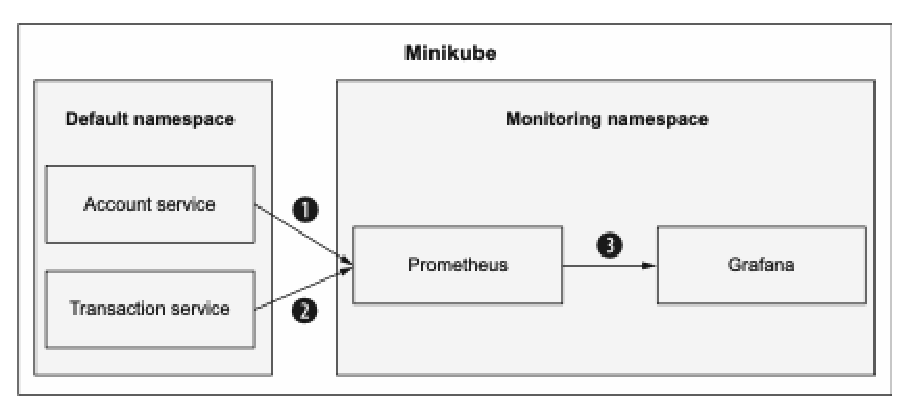
\includegraphics[width=.7\textwidth]{images/5-metrics/prom graf flow.pdf}
    \caption{Prometheus-Grafana Flow.}
    \label{fig:pr_gr_flow}
\end{figure}

Come dette nella Sezione~\ref{sec:prometheus} l'installazione all'interno del cluster Minikube è stata fatta con il chart di Helm \textit{kube-prometheus-stack}~\cite{prometheus_stack}, che comprende sia Prometheus che Grafana.